\documentclass[a4paper,11pt]{article}

\usepackage{préambule}

\newcommand{\exerciceSpacing}{2em}

\begin{document}

\begin{center}
	\LARGE
	\uline{Activité : Introduction à Scratch}
\end{center}

\begin{greybox}[frametitle={Pour commencer}]
	Pour lancer Scratch : cliquer sur le menu démarrer, puis rechercher 'scratch'. Lancer le programme 'Scratch 2'. \vspace{1em}

	\includegraphics[width=\textwidth]{Images/panneau scratch 2 - annoté.jpg}

	\begin{enumerate}
		\item Pour changer la langue.
		\item Panneau des \textbf{blocks}.

		      Certains blocks on des zones dans lesquelles on peut écrire, comme 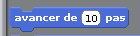
\includegraphics[width=5em]{Images/Block avancer de 10 pas.png}.
		\item Panneau des \textbf{scripts}.
		\item Bouton 'démarrer' et 'stop'.
	\end{enumerate}
\end{greybox}

\vspace{\exerciceSpacing}

\begin{exercice}
	Pour lancer un programme, il \uline{faut} utiliser un block \textit{Évènement}, en jaune. Place le block drapeau (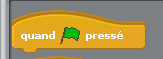
\includegraphics[width=5em]{Images/Block drapeau.png}) dans le panneau des scripts. \\

	Puis, expérimente avec les block d'\textit{Apparence} violets : place en 1 ou plus sous le block drapeau, et décrit ce qu'il se passe :
	\begin{itemize}
		\item Quel est l'effet du block \squared{Dire Salut!} ? Que se passe-t-il si on met un block \squared{Dire Salut!} suivi de \squared{Dire Bonjour!} ? \vspace{0.5em}

		      \dotfill
		\item Quel est l'effet du block \squared{modifier la taille par 10} ? Essayer en remplaçant le nombre par 20, puis par 100. \vspace{0.5em}

		      \dotfill
		\item Quel est l'effet du block \squared{mettre la taille à 100\%} ? Essayer en remplaçant le nombre par 200, puis par 50. \vspace{0.5em}

		      \dotfill
	\end{itemize}
\end{exercice}

\vspace{\exerciceSpacing}

\begin{exercice}[: Boucles]
	Grâce au blocks de \textit{Contrôle} oranges, on peut faire en sorte qu'une action soit effectuée plusieurs fois de suite. \vspace{1em}

	Utilise ces blocks pour que ton personnage suive la souris.
\end{exercice}

\end{document}